%%%%%%%%%%%%%%%%%%%%%%%%%%%%%%%%%%%%%%%%%%%%%%%%%%%%%%%%%%%%%%%%%%%%%%%
%% Related Work
\section{Laboraufbau}
\label{sec:basic-aufbau}
    
Dieses Kapitel befasst sich mit dem Aufbau der Versuchsanlage und der verwendeten Hardware. Dabei werden die Aspekte des räumlichen Aufbau genauso betrachtet wie die Netzwerkinfrastruktur und die genutzten Roboter und Sensoren.



\subsection{Aufbau Teststand}
Der Aufbau vom Teststand ist in den beiden Abbildungen \ref{fig:basic-aufbau-teststand} in der Draufsicht und \ref{fig:basic-aufbau-teststandh} in der Seitenansicht dargestellt. Rote Flächen stellen die Wände dar. Tische sind in blau gezeichnet. Die grüne Fläche ist die Arbeitsplatte auf welcher der Roboter \textit{Dummy} (orange) fixiert ist. Türkise Objekte stellen Geräte wie Kameras und Monitore dar.

 \begin{figure}[H]
 	\centering
 	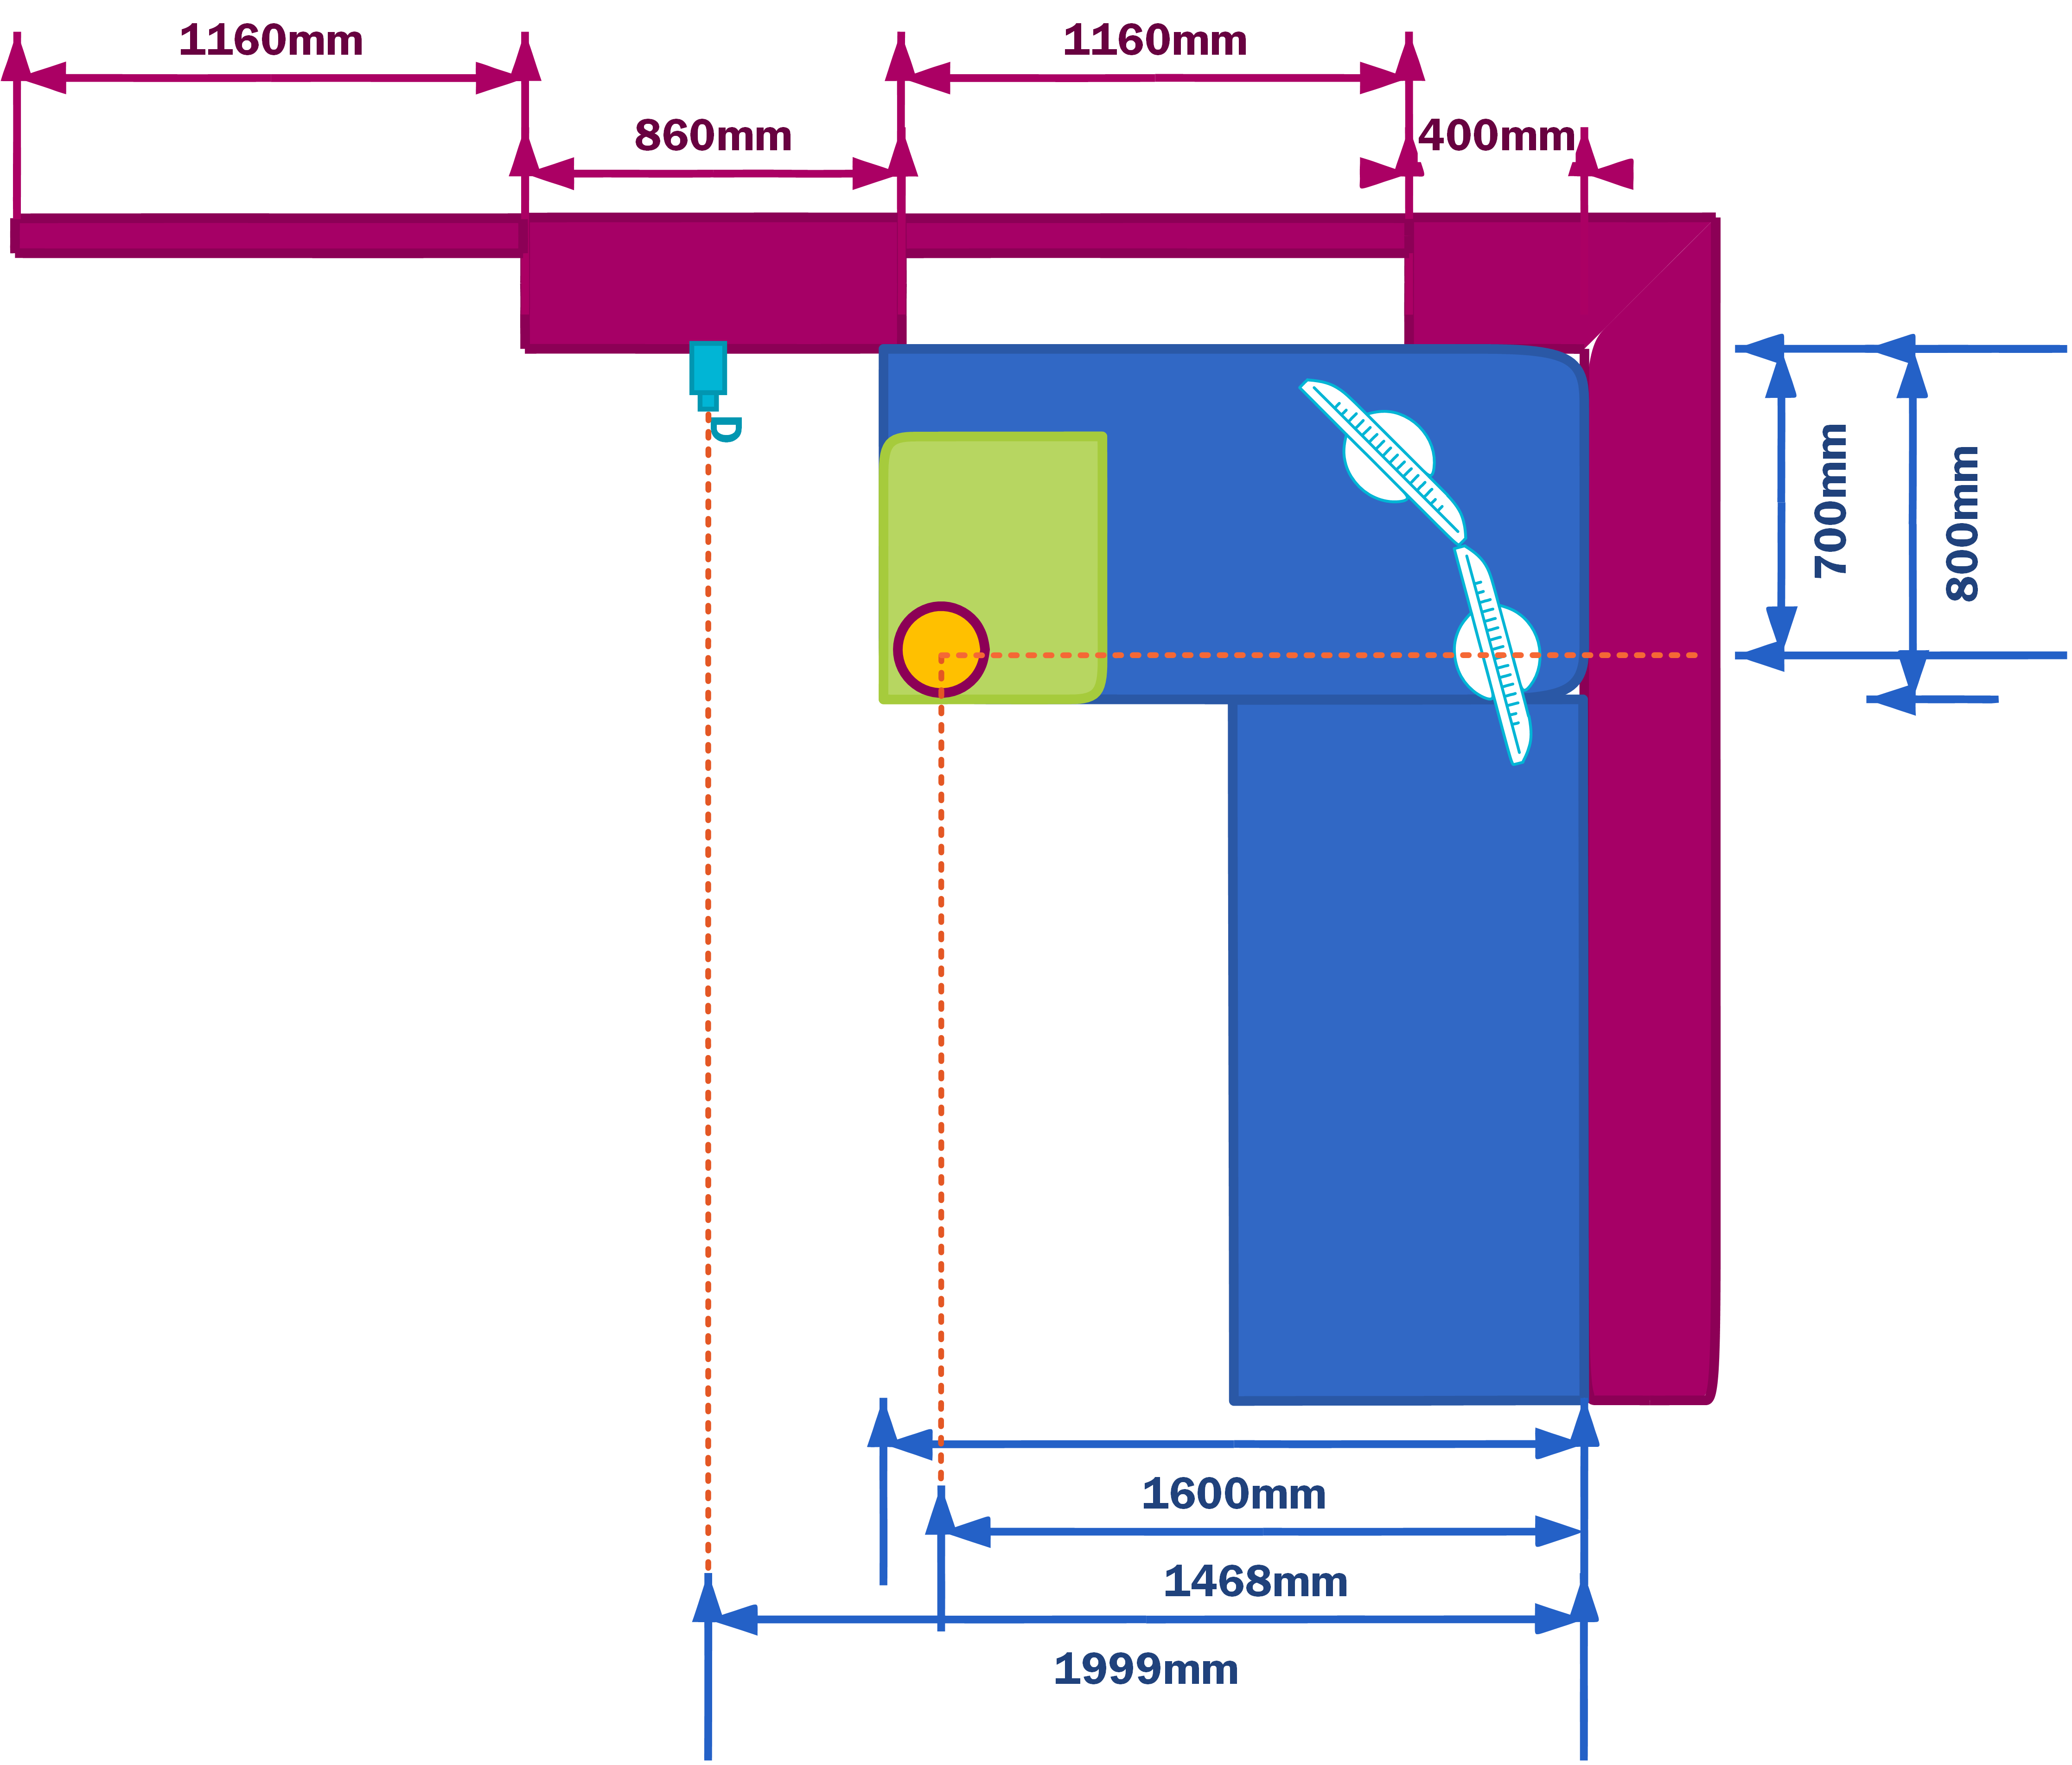
\includegraphics[scale=0.8]{fig/ZeichnungRaum}   
 	\caption[Aufbau Teststand: Draufsicht]{Der Aufbau aus der Draufsicht vom Teststand. Rot: Wände, Blau: Tische, Grün: Arbeitsplatte Roboter, Orange: Roboter, Türkis: Geräte}
 	\label{fig:basic-aufbau-teststand}
 \end{figure}
 
 
 
  \begin{figure}[h]
  	\centering
  	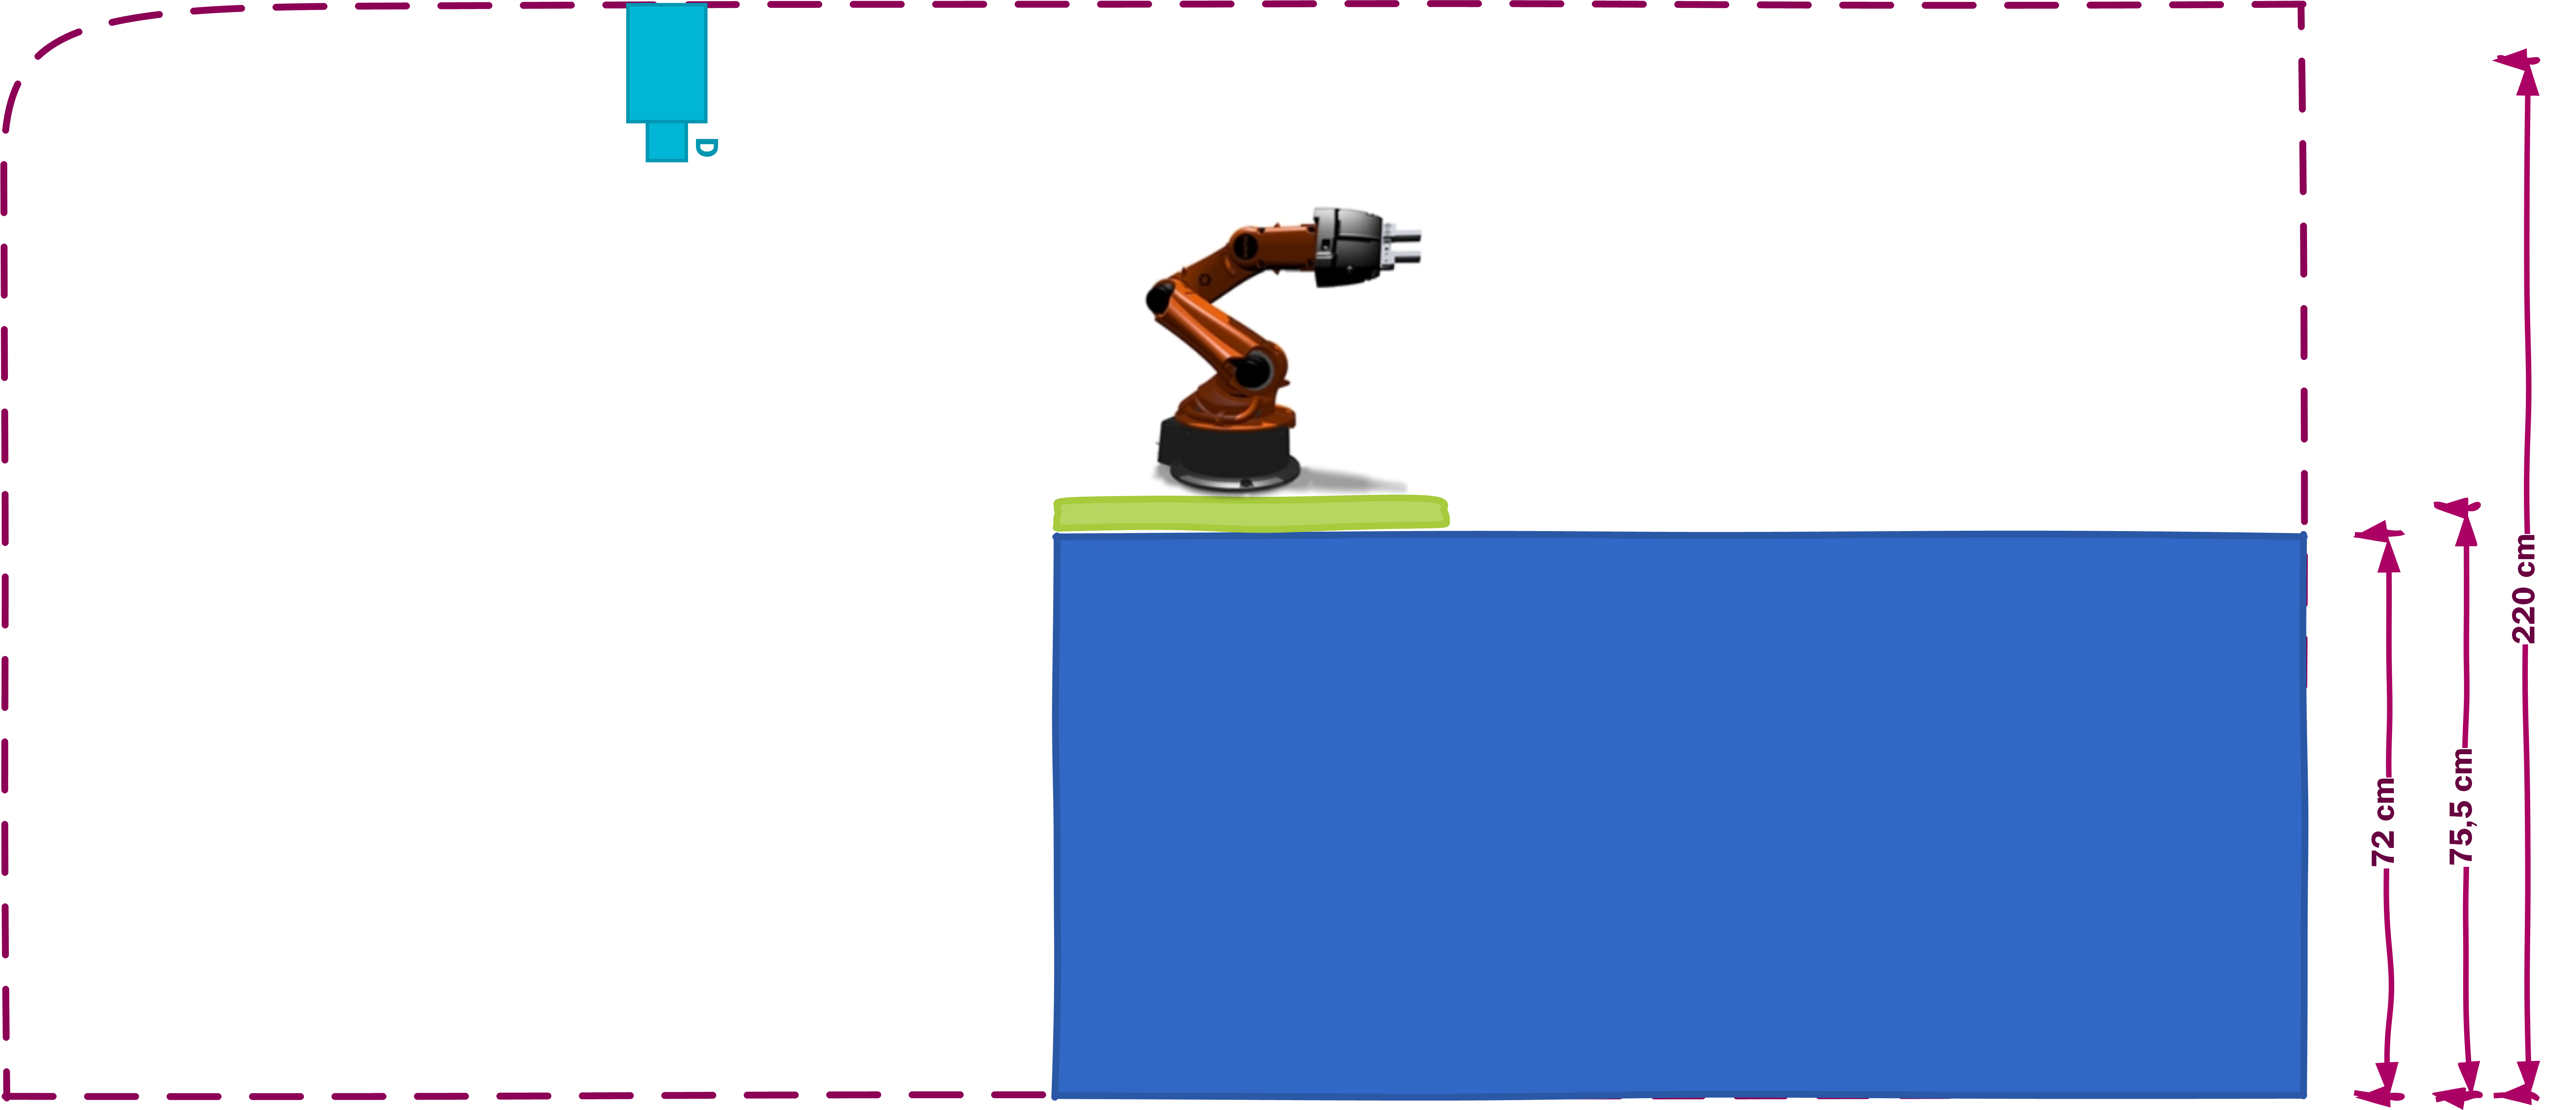
\includegraphics[scale=0.5]{fig/ZeichnungRaumH}   
  	\caption[Aufbau Teststand: Seitenansicht]{Der Aufbau aus der Draufsicht vom Teststand. Rot gestrichelt: Wände, Blau: Tische, Grün: Arbeitsplatte Roboter, Orange: Roboter, Türkis: Kamera}
  	\label{fig:basic-aufbau-teststandh}
  \end{figure}

\subsection{YouBot}
In dieser Arbeit werden zwei Roboter genutzt. Bei beiden handelt es sich um YouBots der Firma Kuka. Diese wurden 2010 erstmals auf der Automatica in München vorgestellt. Kuka ist ein deutscher Hersteller von Industrierobotern mit Sitz in Augsburg.Kuka hat aber auch Erfahrung im Bau von experimentellen Robotern wie etwas die Arme für Justin, einem Service-Roboter.

Die beiden YouBots unterscheiden sich beim Aufbau. YouBot 1 besteht aus einem Manipulator mit Gripper, YouBot 2 besteht aus Manipulator mit Gripper und mobiler Plattform mit omnidirektionalen Rollen. Zur besseren Unterscheidung und zur Lesbarkeit dieser Arbeit haben beide Roboter einen Namen bekommen. YouBot 1 entspricht dabei \textbf{Dummy}, YouBot 2 ist \textbf{Rose}. Im Weiteren Verlauf der Arbeit werden nur noch diese Namen genutzt um eine Verwechslung zu vermeiden.


\subsubsection{Manipulator}
 Die Roboterarme von Dummy und Rose sind eine offene kinematische Kette mit fünf Joints, die von der Basis aufsteigend numeriert sind. An Joint 5 sind die Gripper montiert, diese bestehen aus zwei individuellen Fingern, die linear auf einer Achse bewegt werden können.

Joint 1 und Joint 5 sind zwei Drehgelenke um die Z-Achse, die bei ausgestreckter Haltung (Candle-Pose) parallel liegen. Joint 2, 3 und 4 sind Kippgelenke um die X-Achse, die immer parallel liegen. Durch diese Konstellation ergeben sich für den kompletten Arm fünf Freiheitsgrade (5-DOF). Durch die Einschränkung der Achsen auf die X- und Z-Achsen der einzelnen Joints ist ein seitlicher Griff bei $x_{base} = 0$ oder $y_{base} = 0$ nicht möglich. Die Höhe in Candle-Pose beträgt inklusiv Gripper 655mm. Die einzelnen Abstände lassen sich der Grafik \ref{fig:basic-aufbau-youbot-kinematik} entnehmen.

\begin{figure}[H]
	\centering
	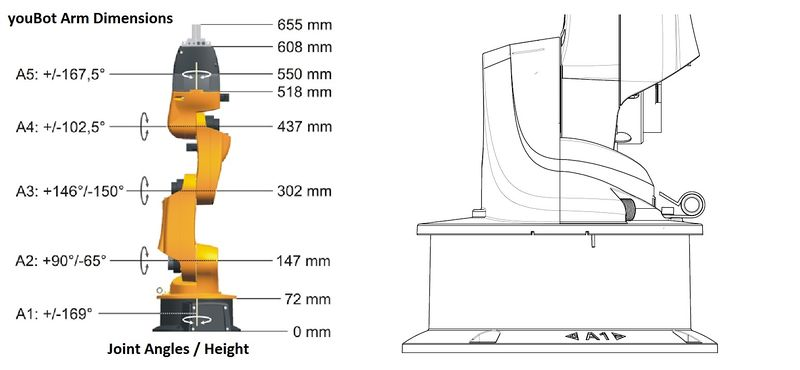
\includegraphics[scale=0.8]{fig/kukaarm_1}   
	\caption[YouBot Arm Kinematik]{YouBot Arm Kinematik. Links: Detailierter Mechanismus mit Joint und Link Angaben. Rechts: Vergrößerte Darstellung der Basis. Bildquelle: \cite{monikaflorekjasinska2015}}
	\label{fig:basic-aufbau-youbot-kinematik}
\end{figure}



 
 Tabelle \ref{tab:basic-aufbau-youbot-joints} stellt noch einmal den Drehbereich aller Joints dar. Dabei sind neben Bezeichner auch die minimalen und maximalen Winkel, sowie die Winkelgeschwindigkeiten. Eine Besonderheit stellt Joint 3 dar, durch den Aufbau bedingt wurde die Achse innerhalb der Treiber gespiegelt, sodass die Winkel um den 0° Punkt gespiegelt wurden. In der Tabelle und den folgenden Zeichnungen ist diese Spiegelung nicht beachtet.
 
   \begin{table}[H]
   	\begin{tabular}{|c|c|c|}
   		\hline Bezeichnung & Max./Min. Winkel & Winkelgeschwindigkeit (rad / s) \\ 
   		\hline Joint 1 & $\pm$ 2.94 & $\frac{\pi}{2}$  \\ 
   		\hline Joint 2 & + $\frac{\pi}{2}$ / -1.13  & $\frac{\pi}{2}$ \\ 
   		\hline Joint 3 & +2.54 /-2.63 & $\frac{\pi}{2}$ \\ 
   		\hline Joint 4 & $\pm$1.78 & $\frac{\pi}{2}$ \\ 
   		\hline Joint 5 & $\pm$2.91 & $\frac{\pi}{2}$ \\ 
   		\hline 
   	\end{tabular}
   	\caption[YouBot Arm Joints]{YouBot Arm Joints. Quelle: \cite{monikaflorekjasinska2015}}
   	\label{tab:basic-aufbau-youbot-joints}
   \end{table}
   
   Der Arbeitsraum des YouBot Arms beschränkt sich durch die Joints. Die Grafiken \ref{fig:basic-aufbau-youbot-workspace} und \ref{fig:basic-aufbau-youbot-workspace-top} stellen den Arbeitsbereich eingeschränkt dar. Die Darstellung \ref{fig:basic-aufbau-youbot-workspace} zeigt mit Hilfe von Konturen die einzelnen Bahnen unter Beschränkung der Joints, sowie der End-Effektor Ausrichtung.  Die äußerste Kontur gibt die maximale Reichweite für den End-Effektor an. Die Z-Achse steht dabei orthogonal zur Tangente an der Konturposition. Abbildung \ref{fig:basic-aufbau-youbot-workspace-top} gibt eine Draufsicht auf den Arbeitsraum. Durch die Beschränkung von Joint 1 befindet sich ein toter Winkel im "Rücken" der Arms. Dieser kann durch einen Überschlag des ganzen Arm, insbesondere Joint 2 und 3, und einer 180 \textdegree Drehung von Joint 1 dennoch erreicht werden. Dies wird durch den linken Bereich in Abbildung \ref{fig:basic-aufbau-youbot-workspace} klar.
   
   \begin{figure}
   	\centering
   	\subfigure[YouBot Arm Arbeitsraum. Reichweite der einzelnen Gelenk und einzelne Abmessung der Links und Link-Offsets. Einheitslose Angaben sind in mm.]{%
   		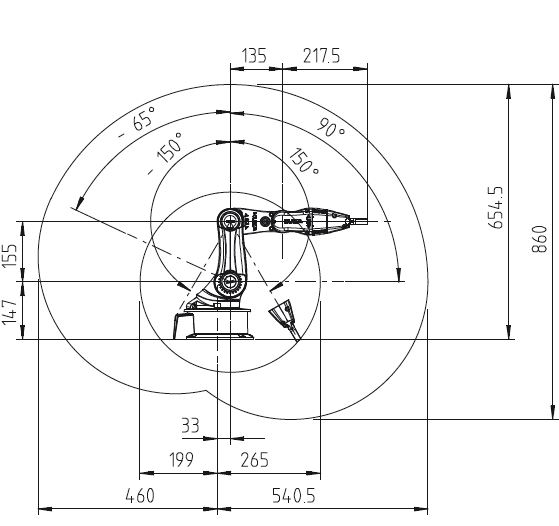
\includegraphics[scale=0.55]{fig/kukaarm_2}
   		\label{fig:basic-aufbau-youbot-workspace}}
   	\hfill
   	\subfigure[Draufsicht YouBot Arm Arbeitsraum.]{%
   		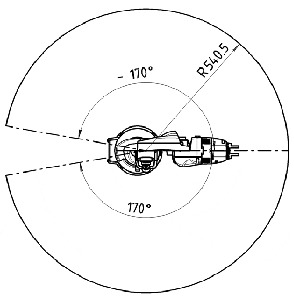
\includegraphics[scale=0.55]{fig/kukaarm_3}
   		\label{fig:basic-aufbau-youbot-workspace-top}}
   	\caption{Arbeitsraum YouBot. Bilderquelle:\cite{monikaflorekjasinska2015}}
   	\label{fig:basic-aufbau-youbot-workspace-full}
   \end{figure}

\subsubsection{Mobile Plattform}
Rose besitzt neben dem Arm noch eine mobile Plattform. Diese ist 590 mm lang, 380 mm breit und 140 mm hoch. Die Plattform hat vier Räder mit einem Durchmesser von 47.5 mm. Jedes Rad lässt sich getrennt ansteuern. Bei den Rädern handelt es sich um Mecanum-Räder, die eine Steuerung in alle Richtungen ermöglicht. Dazu sitzen auf jeder Felge sechs drehbare tonnenförmige Rollen die im Winkel von 45° zur Achse des Rades angebracht sind. Damit Omni-Direktionale Bewegungen möglich sind werden die Räder abwechselnd zum Nachbar auf +45° oder -45° angeordnet. Die minimale Geschwindigkeit der Plattform beträgt $0.01\frac{m}{s}$, die maximale  $0.8\frac{m}{s}$. Abbildung \ref{fig:basic-aufbau-youbot-base} zeigt den Aufbau und Abmessungen der Plattform. 

\begin{figure}[H]
	\centering
	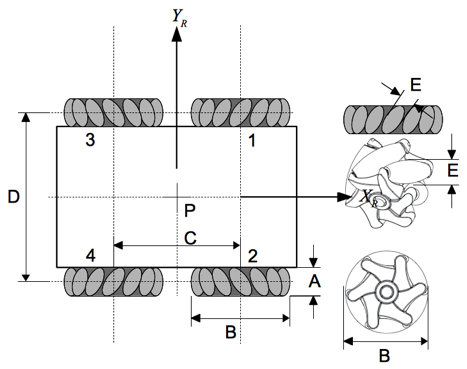
\includegraphics[scale=0.8]{fig/kukabase}   
	\caption[YouBot Base]{YouBot Base. A = 74.87 mm, B = 100 mm, C = 471 mm, D = 300.46 mm E = 28 mm. Die Bodenfreiheit der Plattform beträgt 20 mm. Bildquelle: \cite{monikaflorekjasinska2015}}
	\label{fig:basic-aufbau-youbot-base}
\end{figure}

Die Plattform von Rose ist modifiziert und besitzt eine Aufsatzplatte. Diese dient zur Montage zusätzlicher Sensoren und zur Schutz der Räder bei Kollisionen. Diese ist 600 mm lang und 396 mm breit. Durch die Abstandsbolzen und die Dicke der Platte (5 mm) erhöht sich die Plattform auf 150 mm (siehe Abbildung \ref{fig:basic-aufbau-youbot-base_side}).  

 \begin{figure}[H]
 	\centering
 	\subfigure[Seitenansicht mobile Plattform mit Sensorplatte]{%
 		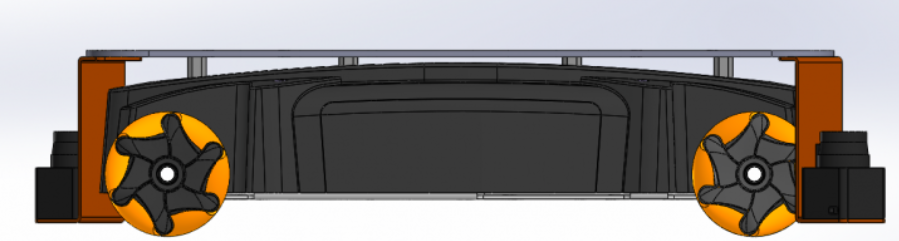
\includegraphics[scale=0.55]{fig/base2}
 		\label{fig:basic-aufbau-youbot-base_side}}
 	\subfigure[Draufsicht mobile Plattform mit Sensorplatte]{%
 		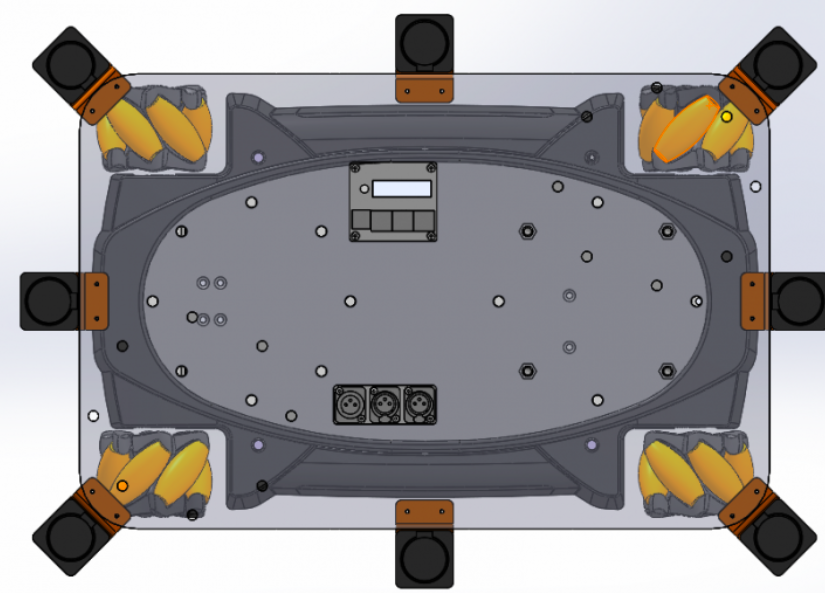
\includegraphics[scale=0.55]{fig/base3}
 		\label{fig:basic-aufbau-youbot-base-top}}
 	\caption{Mobile YouBot Plattform mit Sensorplatte. Bilderquelle:\cite{kuka2015}}
 	\label{fig:basic-aufbau-youbot-base-full}
 \end{figure}

\subsubsection{Rechner}
Für die Rechenleistung der beiden Roboter sorgen neben den verbauten, eingebetteten Boards zwei Computer mit Linux Betriebssystemen.
Der für Rose zuständige PC ist ein Mini-ITX und in der mobilen Plattform eingebaut. Dieser läuft mit einem Intel Atom D510 Dual Core mit 1.66 GHz als CPU und 2 GB DDR2 RAM. Als Festplattensystem ist eine 32 GB SSD verbaut. Der Rechner stellt einige IO-Schnittstellen zur Verfügung: sechs USB 2.0, ein VGA und zwei LAN Anschlüsse sind nutzbar. Dabei ist ein LAN Anschluss für den Ethercat-Anschluss der Plattform belegt. Diese wiederum bringt nochmal zwei LAN Anschlüsse mit. Der Rechner für Dummy ist ein TODO %TODO Dummy PC

Weitere Details zu den Armen, der Plattform oder den Rechnern befindet sich im Anhang \ref{app:daten}.

\subsection{Sensoren}
\label{sec:aufbau-sensoren}
Für die Erkennung von Objekten und der Positionierung im Raum sind mehrere Sensoren nötig. In dieser Arbeit wird dabei auf das Kamerasystem Asus XTion Pro Live und auf einen Laserscanner Hokuyo URG-04LX-UG01 zurückgegriffen.

\subsubsection{Asus XTion Pro}
Die XTion Pro ist ein Tiefenkamerasystem von Asus. Es besteht aus einer RGB-Kamera, einer Tiefen-Kamera und zwei Mikrophonen. Die Kamera wurde von Prime Sense entwickelt und ist eine um gelabelte Microsoft Kinect. Die XTion ist kleiner und leichter als die Kinect und damit besser für die Robotik geeignet. Angeschlossen wird die XTion mit einem USB Kabel und betrieben mit dem ROS Paket OpenNI2. Der Node published eine PointCloud mit RGB Daten, sowie eine PointCloud für die Tiefenkamera, als auch Bilder der RGB Kamera.

Das Sichtfeld der Kamera beträgt Horizontal 58\textdegree, 45\textdegree Vertikal und 70\textdegree Diagonal. Die Auflösung der Tiefenkamera beträgt bei 30 Frames pro Sekunde 640x480 und bei 60 FPS 320x240. Die Auflösung des RGB-Bildes 1280x1024. Die nutzbare Distanz der Tiefenkamera beträgt zwischen 800 mm und 3500 mm.\cite{asus2015} Diese Distanz schränkt die Nutzbarkeit der Kamera ein, so ist sie nicht für eine visuelle Unterstützung der Gripper geeignet, wenn sie an diesen montiert ist, da die Distanz zwischen Kamera und Gripper kleiner 800 mm ist.

\begin{figure}[H]
	\centering
	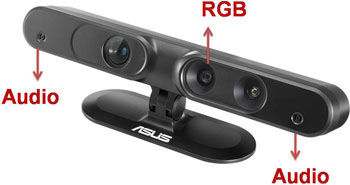
\includegraphics[scale=0.8]{fig/xtion1}   
	\caption[Asus Xtion Pro Live]{Asus XTion Pro Live. Bildquelle: \cite{asus2015}}
	\label{fig:aufbau-xtion}
\end{figure}

\subsubsection{Hokuyo URG-04LX-UG01}
Der URG-04LX-UG01 ist ein optischer Abstandsmesser. Dieser kann Entfernungen in einer zirkulären Ebene messen. Entwickelt wurde er von der Firma Hokuyo, welche neben dem URG noch weitere, ähnliche Sensoren anbietet, die andere Reichweiten und Sichtfelder abdecken. Die Sensoren nutzen zur Messung der Entfernung eine Infrarot-Diode mit einer Wellenlänge von 785 nm. Die Distanz wird mit Hilfe der Phasenverschiebung berechnet. Diese Technik reduziert den Einfluss durch das Oberflächenmaterial des gemessenen Objektes. Versorgt wird der Sensor mit 5V DC, welche über den USB-Anschluss angelegt werden. Da die Startleistung des Sensors die maximale Abgabeleistung eines einzigen USB-Anschluss überschreitet, müssen ein Y-USB-Kabel und zwei USB-Anschlüsse genutzt werden. Angesteuert wird der Sensor mit dem ROS-Paket Hokuyo-Node, welche eine PointCloud published.

Der URG-Sensor hat eine Reichweite von maximal 4000 mm und benötigt für eine Messung 100 ms, was einer Messrate von 10 FPS entspricht. Das Sichtfeld beträgt 240\textdegree. Die minimale Graduelle Auflösung beträgt 0.36\textdegree. Dadurch ergeben sich die ungefähren Disparitäten von 20 mm bei 2000 mm und maximal 40 mm bei 4000 mm Radius. Die Ungenauigkeit beträgt maximal 3 Prozent des gemessenen Wertes, was bei der maximalen Reichweite von 4000 mm einer Abweichung von 120 mm entspricht.\cite{maeda2009}

 \begin{figure}[H]
 	\centering
 	\subfigure[Produktbild. Bildquelle: \cite{nowak2015}]{%
 		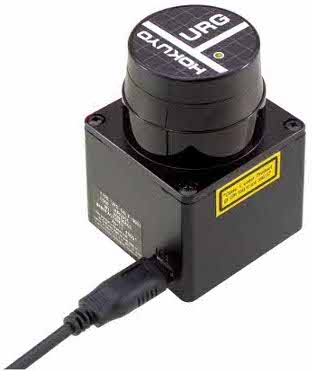
\includegraphics[scale=2.5]{fig/hok2}
 		\label{fig:aufbau-hok2}}
 	\subfigure[Schema: Reichweite und Sichtfeld. Sichtfeld in Messpunktsektoren (MP) unterteilt. Verändert nach: \cite{maeda2009}]{%
 		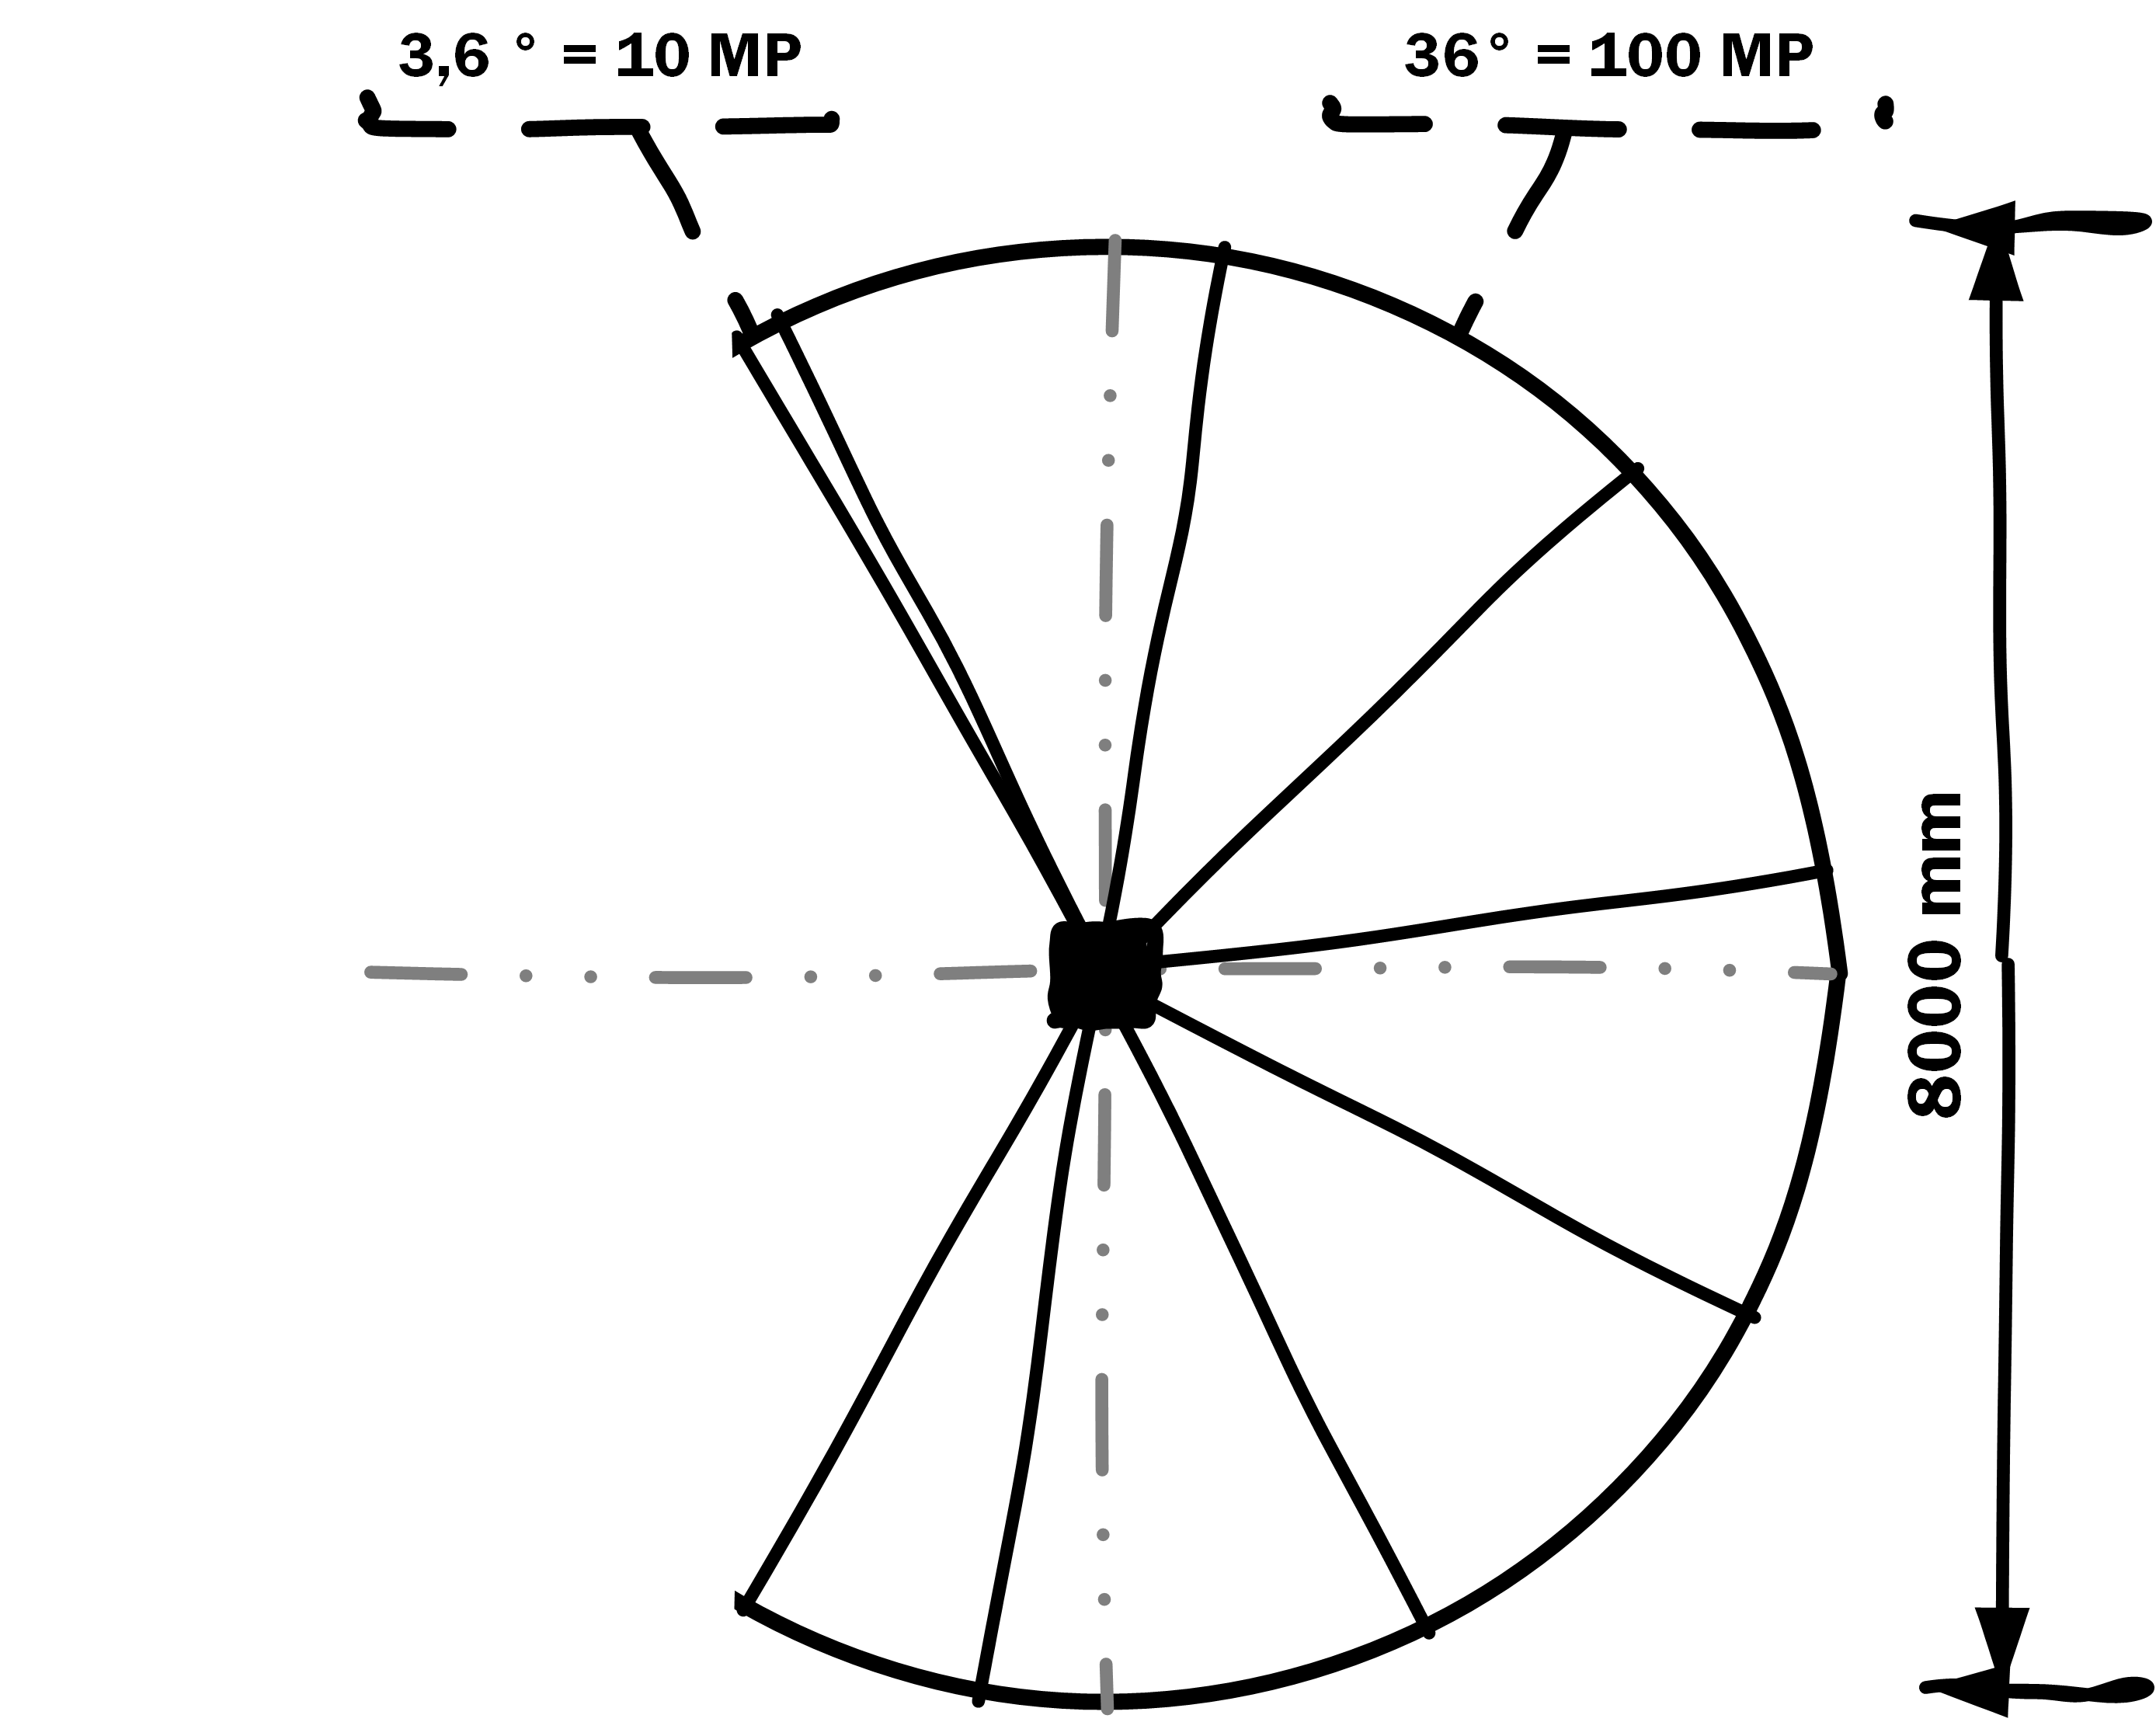
\includegraphics[scale=0.7]{fig/hok1}
 		\label{fig:aufbau-hok1}}
 	\caption{Hokuyo URG-04LX-UG01}
 	\label{fig:aufbau-hok}
 \end{figure}

\subsubsection{Argos 3D - P100}
Ein weiterer Tiefensensor ist die Argos 3D – P100 von Bluetechnix. Diese arbeitet mit dem Time of Flight (ToF) Prinzip. Der Sensor wird mit einem USB-Kabel angesteuert, benötigt aber noch eine weitere Stromzufuhr. Der Sensor kann aus ROS mit einem eigenen Node angesprochen werden. Der Sensor hat eine Reichweite zwischen 100 mm und 3000mm. Die Framerate beträgt bis zu 160 FPS bei ein Auflösung von 160 x120. Das Sichtfeld beträgt 90 \textdegree.\citep{bluetechnix2015}

\begin{figure}[H]
	\centering
	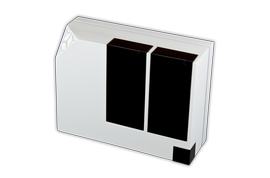
\includegraphics[scale=0.8]{fig/argos3d}   
	\caption[Argos 3D - P100]{Argos 3D - P100. Bildquelle: \cite{bluetechnix2015}}
	\label{fig:aufbau-argos3d}
\end{figure}

\subsubsection{Netzwerk- und Sensoranbindung}

\begin{figure}[H]
	\centering
	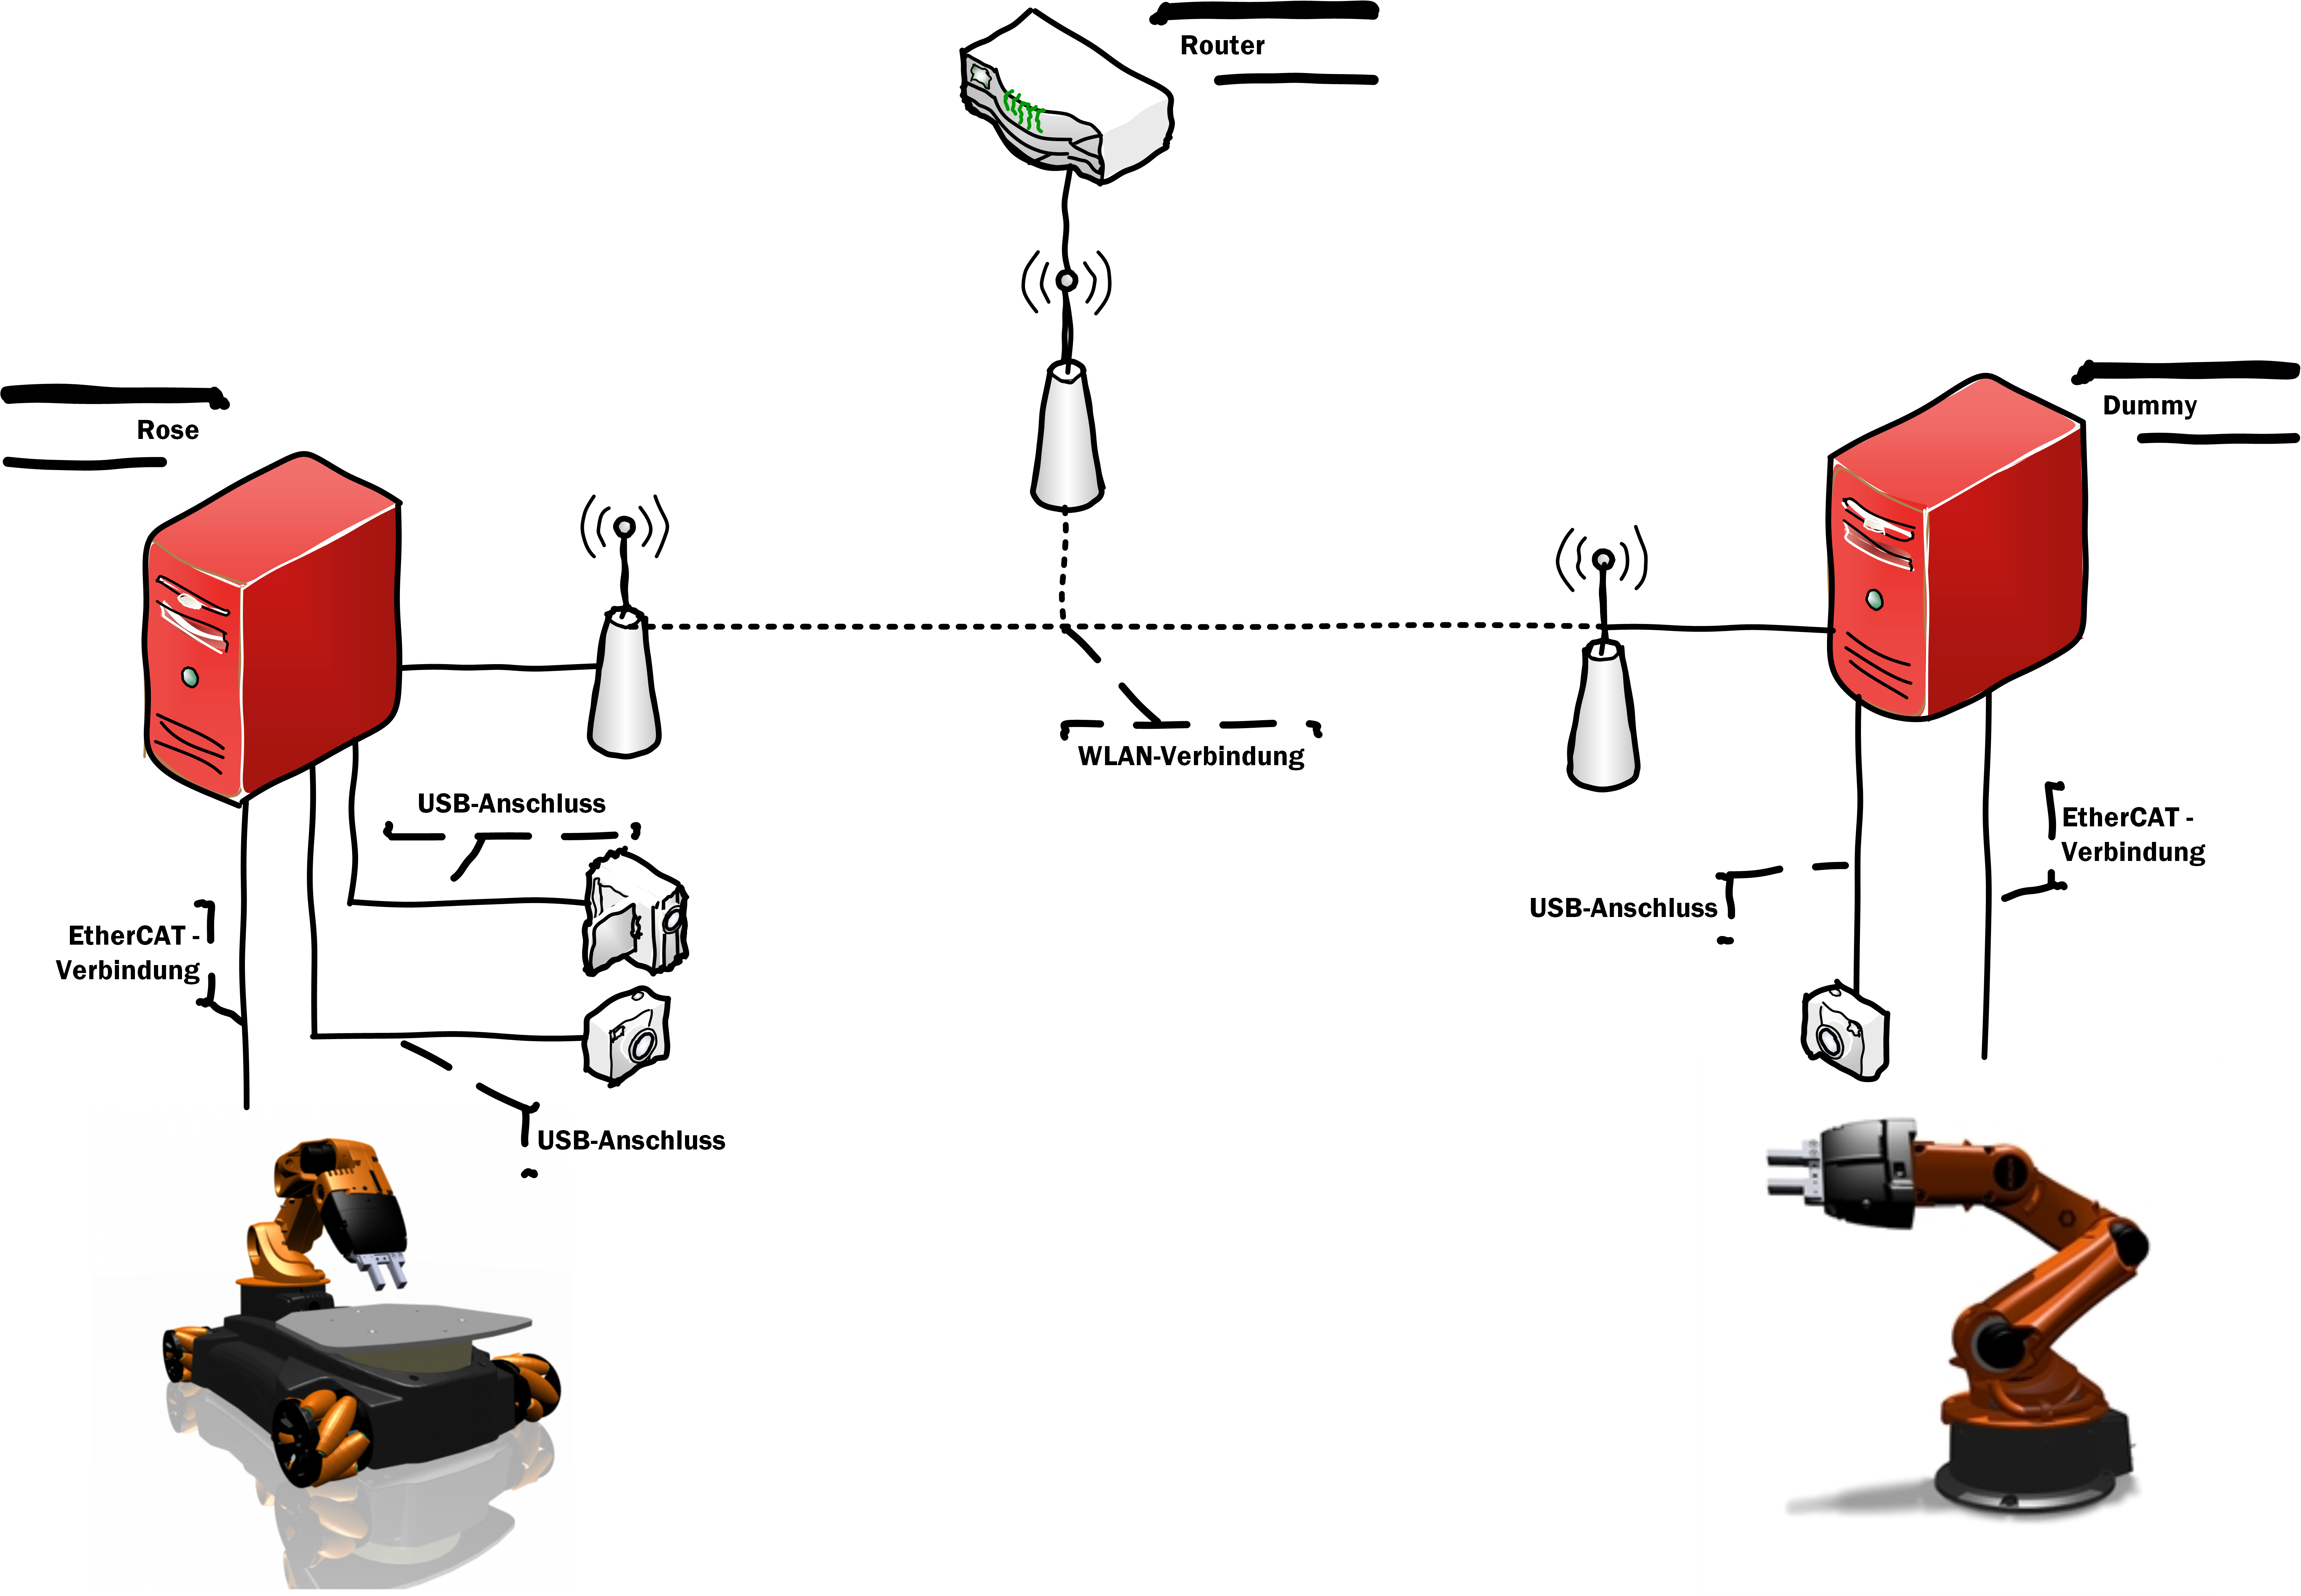
\includegraphics[scale=0.5]{fig/netw}   
	\caption[Schematische Darstellung der Verbindungen]{Schematische Darstellung der Verbindungen}
	\label{fig:aufbau-netw}
\end{figure}

Abbildung \ref{fig:aufbau-netw} stellt den genutzten Verbindungsplan dar. Die zentrale Komponente ist der Router, welcher mit einem externen Access-Point (AP) eine WLAN-Verbindung ermöglicht. Mit diesem WLAN verbinden sich die beiden Steuerungsrechner \textit{Rose} und \textit{Dummy}, welche beide unter diesen Hostnames im Netz erreichbar sind. Die Verbindungen auf beiden Seiten sind gleich gehalten. Die Verbindung zwischen Rechner und Roboter sind mit der EtherCAT-Schnittstelle (Ethernet for Control Automation Technology) realisiert. Diese Ethernet-Variante wurde für Echtzeit-Anforderungen entwickelt, indem Wert auf kurze Zykluszeiten ($\leq$ 100 $\mu$s) und  niedrigem Jitter für exakte Synchronisierung ($\leq$ 1 $\mu$s) gelegt wurde.\cite{ethercat} Die Verbindung zwischen den Rechnern und den Sensoren ist mit USB-Verbindungen umgesetzt. Dabei werden alle USB-Anschlüsse auf der mobilen Plattform von Rose vollständig durch die Sensoren, sowie dem WLAN-USB-Dongle und dem Tastatur/Maus-Dongle belegt. Weitere USB-Geräte sind nur durch einen zusätzlichen HUB möglich. 

Eine Alternative zu diesem Plan ist ein vermaschtes Netz, wie bei PEIS gefordet. Dadurch könnte der Router wegfallen, da alle Endgeräte direkt miteinander verbunden sind. Des Weiteren könnten einige Sensoren auf eigene Rechner ausgegliedert werden. Dies würde die einzelnen Rechner, besonders den leistungsschwachen Rechner von Rose, entlasten, aber auch die Netzwerkkomplexität und die Kosten steigern.